\begin{figure}[htbp]
\centering
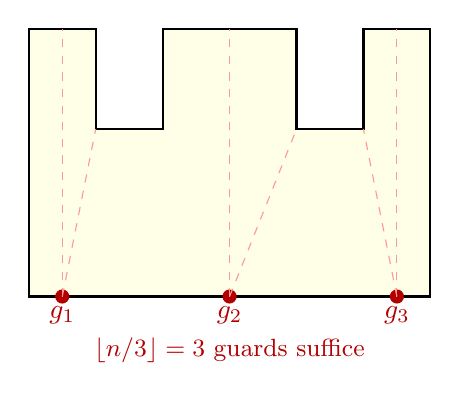
\begin{tikzpicture}[scale=0.85]
  \draw[thick,fill=yellow!10] (0,0)--(6,0)--(6,4)--(5,4)--(5,2.5)--(4,2.5)--(4,4)--(2,4)--(2,2.5)--(1,2.5)--(1,4)--(0,4)--cycle;
  \fill[red!70!black] (0.5,0) circle (3pt) node[below] {$g_1$};
  \fill[red!70!black] (3,0) circle (3pt) node[below] {$g_2$};
  \fill[red!70!black] (5.5,0) circle (3pt) node[below] {$g_3$};
  \draw[red!40,thin,dashed] (0.5,0)--(0.5,4);
  \draw[red!40,thin,dashed] (0.5,0)--(1,2.5);
  \draw[red!40,thin,dashed] (3,0)--(3,4);
  \draw[red!40,thin,dashed] (3,0)--(4,2.5);
  \draw[red!40,thin,dashed] (5.5,0)--(5.5,4);
  \draw[red!40,thin,dashed] (5.5,0)--(5,2.5);
  \node[font=\small,red!70!black] at (3,-0.8) {$\lfloor n/3 \rfloor = 3$ guards suffice};
\end{tikzpicture}
\caption{Art gallery problem: a comb polygon with $n=12$ vertices requires $\lfloor 12/3 \rfloor = 4$ guards in the worst case.}
\label{fig:art_gallery}
\end{figure}
